\documentclass{article}

\RequirePackage{hyperref}

\usepackage[parfill]{parskip}
\usepackage[letterpaper, portrait, margin=1in]{geometry}
% Author
\usepackage{authblk}
% Images
\usepackage{graphicx}
\usepackage{lscape}
\usepackage{longtable}
% \usepackage{svg}

%\articlesubtype{This is the article type (optional)}
% \bibliography{paper-webserver.bib}

\begin{document}

\title{Spfy: an integrated graph-based sequence database for real-time prediction of Escherichia coli phenotypes}

\author[1]{Kevin K Le\thanks{kevin.le@canada.ca}}
\author[1]{Matthew D Whiteside}
\author[1]{James Hopkins}
\author[1]{Victor PJ Gannon}
\author[1]{Chad R Laing\thanks{chad.laing@canada.ca}}
\affil[1]{National Microbiology Laboratory at Lethbridge, Public Health Agency of Canada, Twp Rd 9-1, Lethbridge, AB, T1J 3Z4, Canada}

\renewcommand\Authands{ and }

\maketitle

\begin{abstract}

Current comparative computational workflows chain different analysis software, but lack storage and retrieval methods for generated results.
Spfy uses graph data structures to store and retrieve results for computational workflows, facilitating the management and querying of tens of thousands of whole-genome \textit{E. coli} sequences, and efficient downstream processing.
By making the storage and retrieval of results part of the platform, with data effectively linked to the organisms of interest through a standardized ontology, we can mitigate the recomputing of analyses.
Within Spfy, the output from all analyses is stored, and linked together in the context of a genome graph. This graph also stores metadata for each genome, facilitating inquiries ranging from population genomics to epidemiological investigations.
Integrated data storage will be necessary as publicly available whole genome sequencing data for bacterial pathogens currently numbers in the tens of thousands, with hundreds of thousands set to be available within the next few years. \par

The database is available at \url{https://lfz.corefacility.ca/superphy/spfy/}.

\end{abstract}


\section{Introduction}
% new outline
% para
% 1. brief: WGS is standard
% 2. Big Problem: but tools are for individual analysis
% 3. 100,000 genomes, (lookup number for Enterobase, GenBank), how do we run analysis on it
% 4. previous methods (Galaxy/IRIDA: real-time, but no storage of results, other website examples - Denmark?), what problems they addressed
% 5. Problems that remain / lack of result storage means: recomputation, lost data, can't reference old analyses, not suited for "big data"
% 6. Solutions in general: store and increment, huga "big data" analyses, parallelization /queues
% para
% 1. Our specific problem, previous work
% 2. Why solving it is important (for Public health / research)
% 3. how we solved it
% para
% 4. benefits: rapid analyses in real-time -> huge comparisons, replace reference labs -> time & money saved, future work -> expand analyses, more genomes, more species
% 5. analyses modules -> conda -> IRIDA/Galaxy
% 6. short snippit on website link & github link

% 1. brief: WGS is standard
Whole genome sequencing (WGS) can in theory provide the entire genetic content of an organism. This unparalleled resolution and sensitivity has recently transformed public-health surveillance and outbreak response \cite{ronholm2016navigating,lytsy2017time}. Additionally, the identification of novel disease mechanisms \cite{wang2014whole,yuen2015whole}, and rapid clinical diagnoses and reference lab tests based on the specific mechanism of disease are now possible. \cite{willig2015whole,dewey2014clinical}.

% 2. Big Problem: but tools are for individual analysis
The rapid characterization and comparison of bacterial pathogens relies principally on the combination of outputs from multiple software programs that are targeted for specific applications. Examples include the Resistance Gene Identifier (RGI) \cite{mcarthur2013comprehensive} for antimicrobial resistance (AMR) gene prediction, VirulenceFinder \cite{kleinheinz2014applying} for virulence factor (VF) annotation, and Prokka for bacterial genome annotation with external tools \cite{doi:10.1093/bioinformatics/btu153}. In particular, RGI and VirulenceFinder represent a series of \textit{in-silico} methods which have been developed to replicate the results of traditional wet-lab tests; this allows new WGS results to be viewed in the context of historical tests.

Comprehensive platforms that combine individual programs into a cohesive whole also exist. These include free platforms such as the Bacterium Analysis Pipeline (BAP) \cite{thomsen2016bacterial}, the Integrated Rapid Infectious Disease Analysis (IRIDA) project \url{http://www.irida.ca/}, and PATRIC \cite{wattam2013patric}. Commercial applications, such as Bionumerics, which is used by PulseNet international for the analyses of WGS data in outbreak situations also exist, and offer support as well as accredited, standardized tests \cite{swaminathan2001pulsenet}.

% 3. 100,000 genomes, (lookup number for Enterobase, GenBank), how do we run analysis on it
Traditionally, these platforms have been applied to samples numbering only a few dozens while WGS data for bacterial pathogens of public health importance have recently accumulated in public databases in the tens of thousands, with hundreds of thousands set to be available within the next few years. For \textit{Escherichia coli}, there are over sixty thousand publicly available genomes in EnteroBase \url{https://enterobase.warwick.ac.uk/} and three million whole genomes in GenBank \cite{doi:10.1093/nar/gks1195}.

Many of the comparative analyses that are run are broadly useful, and therefore computed multiple times. To begin to compute results on all available genomes, an effective method to mitigate the recomputing of analyses is to make the storage and retrieval of results part of the platform, and effectively linked to the organisms of interest with a standardized ontology. Such measures can help ensure the rapid response times required for public health applications, and allow results to be integrated and progressively updated as new data becomes available.

% 4. Our specific problem, previous work
We have previously developed Superphy \cite{whiteside2016superphy}, an online predictive genomics platform targeting \textit{E. coli}. Superphy integrates pre-computed results with domain-specific knowledge to provide real-time exploration of publicly available genomes. While this tool has been useful for the thousands of pre-computed genomes in its database, the current pace of genome sequencing requires real-time predictive genomic analyses of tens-, and soon hundreds-of-thousands of genomes, and the long term storage and referencing of these results, something that the original SuperPhy platform was incapable of.

% ?. Why solving it is important (for Public health / research)
% Merging points from here into the above sections (2,3,4) to avoid repetition
% - everything is being sequenced (surveillance / outbreak / research)
% - previously mentioned common analyses / want to leverage pre-computed results
% - WGS does not discard old methods, linkage to thousands of historical results by developing in-silico methods of traditional tests
% - need fast / standardized outbreak response
% - need fast / standardized in-silico reference lab
% - need fast / standardized storage and retrieval of results based on ontology
% - all known data can be leveraged, allows the most informed decisions possible
% - etc.

% 5. how we solved it
In this study, we present the Spfy platform, which integrates a graph database with real-time analysis options. By integrating analysis options with data storage, we avoid recomputing analysis for identical runs. Graph-based result storage also allows retrospective comparisons as more genomes are sequenced or populations change, and is flexible to accommodate new analysis modules as they are developed. The website is available at \url{https://lfz.corefacility.ca/superphy/spfy/}.

% {needs to be beefed up, in language a biologist / public health worker would care about}

% end of new intro

% **************************************************************
% Keep this command to avoid text of first page running into the
% first page footnotes
\enlargethispage{-65.1pt}
% **************************************************************

% Some general comments
% The NAR Database issue is more of a showcase then a rigorous exploration of software design choices.
% Given this focus, i would suggest the following:
% 1. Increase/highlight the discriptions of the functions and capabilities, maybe by adding a Functionality section
% 2. In the Implmentation (or Methods) section, only give a cursory description of the layout and components. Don't need to provide too much justification
% 3. Use the Results section to highlight the scope/size and speed. This can be short
% 4. In the Discussion, this is where i would expand on the justications and reasons for specific design choices. Pick 2-3 main ones and discuss those (i.e. don't need to justify our choice of documentation software). Also compare with other software in Discussion.
% 5. Add a conclusions section


\section{FUNCTIONALITY}
% ONLY FOCUS ON THE ANALYSIS MODULES
% Describe available functions in spfy
% para covering everything

By supporting multiple \textit{in-silico} subtyping options, the platform functions similar to a reference laboratory, while adding support for population analyses. Subtyping options for \textit{E.coli} are O-antigen, H-antigen, and VF gene determination using ECtyper \url{https://github.com/phac-nml/ecoli\_serotyping}, Shiga-toxin 1 (Stx1), Shiga-toxin 2 (Stx2), and Intimin typing using Phylotyper \cite{whiteside2017phylotyper}, and AMR annotation using the RGI program \cite{mcarthur2013comprehensive}.
Spfy also performs bioinformatics analyses: pangenome generation using Panseq \cite{laing2010pan} and support vector machine (SVM)-backed AMR predictions for OmniLog AMR assays using Scikit-learn \cite{pedregosa2011scikit}.

These tasks are divided into subtasks, and distributed across a built-in task queue. Results are converted to individual graphs and stored within a larger graph database. By integrating task distribution with graph storage, Spfy enables large-scale analyses, such as epidemiological associations between specific genotypes, biomarkers, host, source, and other metadata, and statistical significance testing of genome markers for user-defined groups using SciPy \cite{jones2014scipy}. Any data type or relation in the graph is valid for analysis, such as the presence or absence of pan-genome regions against determined serotypes or other subtyping options. In addition, Spfy supports the submission of user-specified metadata, such as location or source information. Currently, the platform has been tested with XXX genome files and result storage for XX analyses modules.

% para covering ectyper & RGI -- don't really need this
% RGI has its own paper and was in the previous SuperPhy paper
% ectyper will get its own paper
% phylotyper also has its own paper

\section{IMPLEMENTATION}
% para: intro to the spfy stack
Spfy's server-side code is developed in Python and the front-end website is developed using the React JavaScript library. For the addition of new data to the database, the following steps are taken:

i) The upload begins through the ReactJS-based website, where user-defined analyses options are selected. The results of these chosen analyses are immediately reported to the user following their completion, while the remaining analyses are subsequently completed and stored in the database without interaction from the user. The public web service accepts up to 200 MB of genome files (50 genomes uncompressed, or 120 genomes compressed) at a time, though an unlimited amount of data can be submitted locally.

ii) User-selected analyses are enqueued into the Redis Queue \url{http://python-rq.org/} task queue. Redis Queue consists of a Redis Database \url{https://redis.io/} and task queue workers which run as Python processes.

iii) The workers dequeue the analyses, run them in parallel, and temporarily store results in the Redis database.

iv) Python functions parse the results and permanently store them in Blazegraph \url{https://www.blazegraph.com/}, the graph database used for Superphy.

\subsection{Data Storage}
% para
% 0. Goals: big-data, everything linked, easy addition of new links
% 1. spfy is built around graph technologies
% 1. how we structure our graph
% 2. ontoogies used
% 3. inferencing
% 3 1/2. SPARQL queries
% para: the semantic web
Semantic web technologies describe the relations between different data \cite{berners2001semantic}. For biological data, individual data points such as genome, contiguous DNA sequence, or gene, can be linked together in a searchable graph structure. This allows novel data to be incorporated into the existing graph, and has the use of graph databases for semantic information has been proposed as a open standard for sharing public information \cite{horrocks2005semantic}. Data points are annotated with terms from published ontologies. To avoid proliferating ontologies, and to allow Spfy to integrate with existing ones, annotations from the GenEpiO \cite{griffiths2017context}, FALDO \cite{bolleman2016faldo}, and TypOn \cite{vaz2014typon} ontologies are used for our annotations.

\begin{figure}[!hb]
\begin{center}
\includegraphics[width=\textwidth]{images/ontology}
\end{center}
\caption{Caption for figure within column.}
\label{fig-ontology}
\end{figure}

% Permanent storage + why a graph is preferable over tables
The permanent storage of results is as a one-time cost to avoid recomputation when the same analysis is re-run. For population analyses, Spfy searches the graph for all data points annotated with the queried ontology term. This graph data is then converted into the required structure, usually numerical arrays, for the given analysis modules.

% TODO: add figure illustrating search.

\subsection{Web design}
% para
% 1. goals: intuitive/familar, ease of use
% 2. design specs
% 3. Google Material design
% 1. implementation: reactjs, react-md, ES6, JSX
% 4. separation from Flask layer

The front-end website is written using the React JavaScript library \url{https://facebook.github.io/react/} as a single-page application resembling a traditional desktop application.
To ensure a familiar user interface, we followed the Material Design specification \url{https://material.io/}, published by Google, surrounding a card-based design.
(see Figure \ref{fig-results})
Both the task selection and result displays follow the same design pattern: while data storage is graph-based, the results of various analysis modules are presented to users in a familiar tabular structure and available for download as .csv spreadsheet files.
(see Figure \ref{fig-tables})

\begin{figure}[!hb]
\begin{center}
\includegraphics[width=\textwidth]{images/results.png}
\end{center}
\caption{Caption for figure within column.}
\label{fig-results}
\end{figure}

\begin{figure}[!hb]
\begin{center}
\includegraphics[width=\textwidth]{images/tables.png}
\end{center}
\caption{Caption for figure within column.}
\label{fig-tables}
\end{figure}

No account creation is required to use the platform. A sharable token is automatically created for users upon opening the website, and is embedded into the website address. Users can share results with their colleagues by copying the URL, and files can be submitted for analysis from different computers with results reflected on each others' screens.

\subsection{Service Virtualization}
% para
% 1. goals: real-time, support for pipelines (linked modules)
% 2. how pipelines have been handled in the past: Galaxy, other examples
% 3. Python, RQ
% para
% 1. how we implemented RQ
%	related: packaging of modules in conda

% para
% 1. goals: scale analyses to "big-data", error handling
% 3. how we handle parallelization with RQ
% para
% 1. how many tasks have we tested this with
% 2. error handling: rq-dashboard, sentry
% 3. why options like sentry are better than traditional logging: scales well to tons (big-data levels) of tasks, groups the same errors together, reporting via email

% para
% 1. goals: why compartmentilizations
% 1. how we implemented docker
% 3. how this lets us replicate worker containers and link everything together

% cost of docker < a full VM
% it's not quite a full OS
Docker \url{https://www.docker.com/} is a virtualization technology to simulate self-contained operating systems on the same host computer, without the overhead of full hardware virtualization \cite{felter2015updated}.
The Spfy platform depends on a series of webservers, databases, and task workers and uses Docker to compartmentalize these services which are then networked together using Docker-Compose \url{https://docs.docker.com/compose/}.
(see Figure \ref{fig-docker})
Docker integration ensures that software dependencies, which are typically manually installed \cite{doi:10.1093/bioinformatics/btu153,laing2010pan,inouye2014srst2,naccache2014cloud}, are instead handled automatically. With compartmentalization of service runtimes, code failures do not propagate to other services.

\begin{figure}[!hb]
\begin{center}
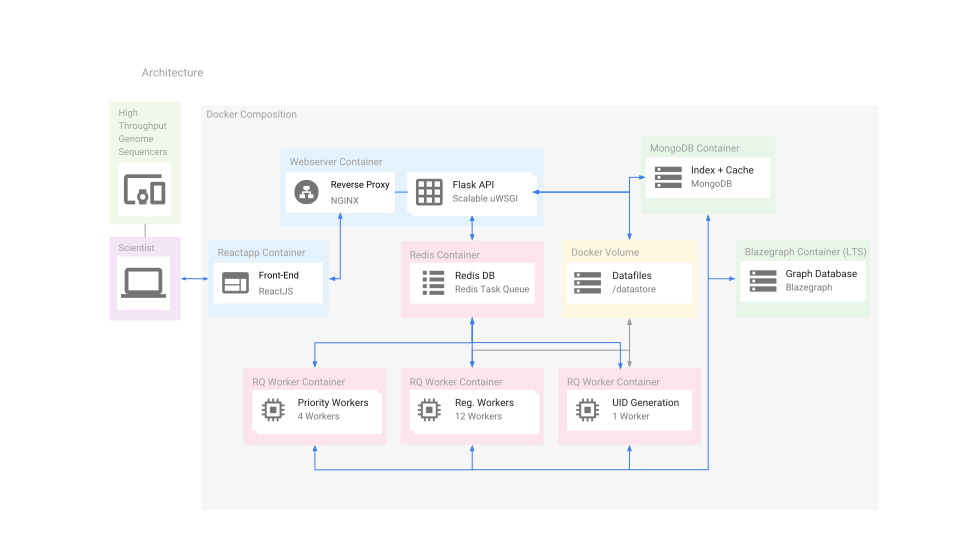
\includegraphics[width=\textwidth]{images/docker}
\end{center}
\caption{Caption for figure within column.}
\label{fig-docker}
\end{figure}

% standard web tech means you can deploy to different cloud computing services
One of the key benefits of using more common-place technologies is the compatibility with other infrastructure resources.
Docker containerization is widely supported by cloud computing services: Amazon Web Services (AWS) \url{https://aws.amazon.com/docker/}, Google Cloud Platform (GCloud) \url{https://cloud.google.com/container-engine/}, and Microsoft Azure \url{https://azure.microsoft.com/en-us/services/container-service/}, and self-hosted cloud computing technologies such as OpenStack \url{https://wiki.openstack.org/wiki/Docker} all support Docker.
% we may want to sign up for a free trial to give an example of this
Spfy packages compute nodes, which manage a collection of task queue workers, as reproducible Docker containers which can be networked together to form a compute cluster.
Docker containerization has a negligible impact on performance \cite{di2015impact}, and allows the platform to easily scale to demand.

\subsection{Continuous integration}
% Keep this short
% para
% 1. goals: why CI, testing is important
% 2. how we've implemented it, integration with github

TravisCI \url{travisci.io}, a continuous integration (CI) platform, is used to ensure that Spfy \url{https://github.com/superphy/backend} does not break with any changes to the codebase, and runs tests for functionality and backwards compatibility.
The individual tests use PyTest \url{https://doc.pytest.org/}, and are run within TravisCI's virtual environment. The current build status can be checked either on our GitHub repository or at \url{https://travis-ci.org/superphy/backend}.
The CI is also used to automatically build Spfy's core Docker images, and upload them to Docker Hub \url{https://hub.docker.com/u/superphy/}.

\section{RESULTS}
Spfy was tested with 10,243 public \textit{E. coli} assembled genomes from Enterobase, storing every sequence and results for all included analysis modules.
All subtyping options: O-antigen, H-antigen, Shiga-toxin 1, Shiga-toxin 2, and Intimin typing, VF and AMR annotation were ran on the reference set. The genomes were also analyzed within the pan-genome framework of \textit{E. coli}, and results from all analyses are automatically associated with the source genome.
The resulting database had 17,820 nodes and 3,811,473 leaves, with 1,125,909,074 object properties. \par

\small % Please add the following required packages to your document preamble:
% \usepackage{graphicx}
\begin{table}[!hb]
\centering
\caption{Database statistics for the various types of nodes, leaves, and associated entries in the graph database, Blazegraph. The database stores all results from every included analysis module and associated metadata. Numbers are representative for analysis of 10,243 assembled genomes.}
\label{Table 1.}
\resizebox{\textwidth}{!}{%
\begin{tabular}{llllllllll}
name               & indexType & m    & height & nnodes & nleaves & nentries  & nodeBytes & leafBytes   & totalBytes  \\
\_\_globalRowStore & BTree     & 32   & 1      & 1      & 6       & 102       & 193       & 8537        & 8730        \\
kb.lex.BLOBS       & BTree     & 692  & 2      & 17     & 6727    & 3227686   & 90596     & 60187016    & 89331537662 \\
kb.lex.ID2TERM     & BTree     & 905  & 2      & 88     & 39912   & 18080577  & 515355    & 293436043   & 2058798455  \\
kb.lex.TERM2ID     & BTree     & 193  & 3      & 1153   & 147978  & 18080577  & 5596557   & 1152764154  & 1158360711  \\
kb.spo.JUST        & BTree     & 284  & 3      & 13213  & 2042532 & 299426518 & 77979362  & 15527483178 & 15605462540 \\
kb.spo.OSP         & BTree     & 708  & 3      & 1649   & 639325  & 262364538 & 11448125  & 3760927987  & 3772376112  \\
kb.spo.POS         & BTree     & 990  & 2      & 864    & 463188  & 262364538 & 8347594   & 2246478879  & 2254826473  \\
kb.spo.SPO         & BTree     & 1024 & 2      & 835    & 471805  & 262364538 & 10308603  & 2661857997  & 2672166600 
\end{tabular}%
}
\end{table}


Spfy has been up since May 2017. The server accepts assembled \textit{E. coli} genomes with the \textit{.fasta} or \textit{.fna} extensions. Submissions are checked against a reference set of \textit{E. coli} gene sequences before running analyses. Outputs are displayed on the website in tables and can be downloaded as \textit{.csv} files. 
\par

% analysis run-time / throughput with different levels of parallelization
% particularly for statistical tests
% should do a 1 genome = X number VFs, Y number of genomes for Y*X retrieval/analysis

\section{DISCUSSION}
% Gist, we address the the "Limitations" of \cite{de2015trends}.
% Namely:
% 1. Custom formats.
% 2. Use of legacy tech (SQL) means youu can't accomadate "Big-Data" goals.

% drawbacks - big data
Many bioinformatics software programs have been developed \textit{ad hoc}, with individual researchers and laboratories developing software specific to their environment \cite{de2015trends}.
Such tools were often script-based, with custom data formats, and only suitable for small collections of data \cite{de2015trends}.
Recent efforts \cite{goecks2010galaxy,thomsen2016bacterial} have focused on providing a common web interface for these programs, while still returning the same result files.
However, many subsets of biology now require the analyses of big-data, where inputs are taken from a variety of analysis programs, and involve large-scale data warehousing \cite{schatz2015biological}.
The ability to perform computations in real-time, store data in flexible databases, and utilize a common application programming interface (API) linking resources are required for these analyses \cite{swaminathan2016review}.

One of the key goals in developing Spfy was to accommodate a variety of result formats, from storing subtyping data to retrieving results as inputs for downstream analyses, such as statistical significance testing. We've shown how a graph database can accommodate a variety of programs used by bioinformaticians and is performant for data retrieval on the results of 10,000+ genomes. Spfy maintains instantaneity, as modern analytics platforms must respond to user-requested analyses of big-data in the same efficiency as old analyses of single files.

\subsection{Impact on Public Health Efforts}

% para
% focus on application
The isolation and characterization of bacterial pathogens are critical for Public Health laboratories to rapidly respond to outbreaks, and to effectively monitor known and emerging pathogens through surveillance programs.
Until recently, public-health agencies relied on laboratory tests such as serotyping, pulsed-field gel electrophoresis (PFGE) banding patterns, or Polymerase Chain Reaction (PCR)-based amplification to identify known VFs or AMR genes, along with other tests \cite{ronholm2016navigating}, to characterize bacterial isolates in outbreak and surveillance settings.

AMR testing, VF testing, and Shiga-toxin testing are of particular importance to surveillance efforts due to their role in a pathogen's lethality.
Current efforts are focused on predictive genomics, where the relevant phenotypic information can be determined through examination of the whole-genome sequence.
WGS methods allow a single laboratory method - the sequencing step - to provide a variety of analysis options, such as AMR, VF, and Shiga-toxin results, and as such can be used to evaluate the spread of outbreaks with better resolution and context than traditional methods \cite{ronholm2016navigating}.

% application: results similar to a wet-lab
Spfy uses WGS results.
After initial sequencing of new isolates, Spfy can be used in place of a traditional reference laboratory, to determine the O-type and H-type, Stx type, and all known VFs and AMR genes in real-time.
These results can be shared with other agencies and researchers over the internet.
Furthermore, using Spfy's database of pre-processed genomes, Spfy can determine all strains a sample may be related to which is useful for monitoring the evolution of pathogens over time.
A computational approach saves the time and cost associated with performing multiple tests per sample, and allows population comparisons to keep pace the current generation WGS data.

\subsection{Comparison with other bioinformatic pipeline technologies}
% trying to cut down on details that would be better suited for the "Implemntation" section.

% namely galaxy
Existing scientific workflow technologies such as Galaxy \cite{goecks2010galaxy}, and pipelines such as the Integrated Rapid Infectious Disease Analysis (IRIDA) platform \url{http://www.irida.ca/} and the Bacterium Analysis Pipeline (BAP) \cite{thomsen2016bacterial} help automate the use of WGS data for public-health surveillance.
Reproducibility is important to science, and Galaxy aims to provide a reproducible, computation-based research environment which is accessible to individuals without programming knowledge. Galaxy defines a formal schema for linking different analysis software together, so analyses can be replicated end-to-end.
Building on top of the Galaxy framework, IRIDA adds prebuilt pipelines specific to bioinformatics uses, as well as sequence and result storage. IRIDA takes a project-based approach, with sequences stored per project, and results stored linearly per whole-genome sequence. Similarly, BAP provides an integrated analysis pipeline for bacterial WGS data as a web service.
For result storage, these workflow technologies either use relational tables \cite{goecks2010galaxy}, or store resulting files to disk \cite{thomsen2016bacterial}.

Like IRIDA and BAP, Spfy automates workflows for users, and like Galaxy, Spfy uses task queues to distribute selected analysis.
% re: Matt "2. When comparing to IRIDA, BAP etc., can mention some differences with Superphy, e.g. the storage of interim result data that allows downstream integrated analysis"
On a per file basis, Spfy performs at a similar speed to BAP on predictive genomics tasks, though Spfy does not provide genome assembly services.
Spfy also processes XXXX files over XX tasks in XXXX time by using a novel approach of distributing computations over a task queue and multiple Docker compartmentalized containers.
We also focus on the data warehousing problem in bioinformatics: storing results as in IRIDA and BAP, but in a way where we can integrate results for further analyses.
Like BAP, Spfy integrates different programs, such as for VF and AMR determination, into one pipeline. 
Because output from these programs is user-specific or transitory, results from identical comparisons are often recomputed. Additionally, output from different analyses are structured using distinct terminology and formats, which must be converted before they can be compared. Without a unified structure, these conversions quickly become impractical for broad usage. Graph-based storage of all results solves these problems.

In place of a relational database for storing the location of result files, Spfy parses and maps results to formal ontologies, with the end result stored in a persistent graph database.
This enables Spfy to create large datasets where analysis results are linked to genomes, and to perform population-wide analyses. In all, Spfy provides similar functionality to IRIDA and BAP with an expanded focus on integrated result storage and big-data analyses.

\section{CONCLUSIONS}

Future work will focus on adding additional analyses modules to aid genotype to phenotype predictions, and supporting different species. We're currently working on an approach using support vector machines to predict \textit{E.coli} phenotypes \url{https://github.com/superphy/kmer} which will be integrated into Spfy. While the integrated approach of storing and retrieving results provides enormous benefits, the developed analyses modules are self-contained and can easily be integrated into existing platforms such as Galaxy \cite{goecks2010galaxy}, and IRIDA. Spfy's codebase is provided at \url{https://github.com/superphy/backend} and a developer guide is provided at \url{https://superphy.readthedocs.io/en/latest/}.

\textit{Conflict of interest}. None declared.

\section{ACKNOWLEDGEMENTS}

\newpage

\bibliographystyle{unsrt}
\bibliography{paper-webserver}

\newpage

\section{APPENDIX}

\end{document}
